\documentclass[border=3pt,tikz]{standalone}
\usepackage[utf8]{vietnam}
\usetikzlibrary{calc,angles,intersections,shapes.geometric,arrows,decorations.markings,arrows.meta,patterns.meta,patterns}
\usepackage{tikz-3dplot,pgfplots}
\pgfplotsset{compat=1.15}
\usepgfplotslibrary{polar}
\usepackage{amsmath}
\begin{document}
	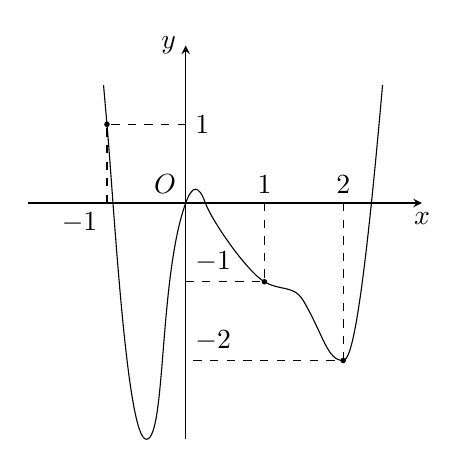
\begin{tikzpicture}
	\draw[-stealth] (-2,0)--(0,0)node[above left]{$O$} --(3,0)node[below]{$x$};
	\draw[-stealth] (0,-3)--(0,2)node[left]{$y$};
	\draw[dashed]
	(-1,0)node[below left]{$-1$}|-(0,1)node[right]{$1$}
	(1,0)node[above]{$1$}|-(0,-1)node[above right]{$-1$}
	(2,0)node[above]{$2$}|-(0,-2)node[above right]{$-2$}
	;
	\draw
	($(-1,1)+(95:.5)$)--(-1,1) .. controls +(-85:1) and +(180:.25) .. (-.5,-3)
	.. controls +(0:.25) and +(-110:1) .. (0,0)
	.. controls +(70:.25) and +(110:.25) .. (.25,0)
	.. controls +(-70:.25) and +(150:.25) .. (1,-1)
	.. controls +(-30:.25) and +(120:.25).. (1.5,-1.25)
	..controls +(-60:.5) and +(180:.2) .. (2,-2)
	.. controls +(0:.1) and +(-95:3) .. (2.5,1.5)
	;
	\fill[black] (-1,1) circle (1pt) (1,-1) circle (1pt) (2,-2) circle (1pt);
\end{tikzpicture}
\end{document}